\SSbreak\\
\emph{Source: AMOC December 2020 Camp Exam 2 (A/G) P4}\\
\emph{Proposer: \Pchris}\\ %\Pchan \Pbrain \Pss
\emph{Problem ID: 130}\\
\emph{Date: 2021-02-12}\\
\emph{Difficulty: Hard}\\
\SSbreak

\SSpsetQ{
Let ABC be a triangle with side lengths AB = 4, BC = 5, CA = 6. Suppose P is a point inside ABC such that the circumcenters B' and A' of triangles ACP and BCP respectively lie outside ABC, with A, P, A' collinear and B, P, B' collinear. The line through P parallel to AB meets the circumcircles of ACP and BCP at E and D respectively, where D, E, P are distinct. 
Suppose \(DE^2 - AP = (a - sqrt(b))/c\) where a, b, c are integers and b is squarefree. Find a + 69b + 420c.
}\bigskip

\begin{solution}\hfil\medskip
  
    \begin{figure}
        \centering
        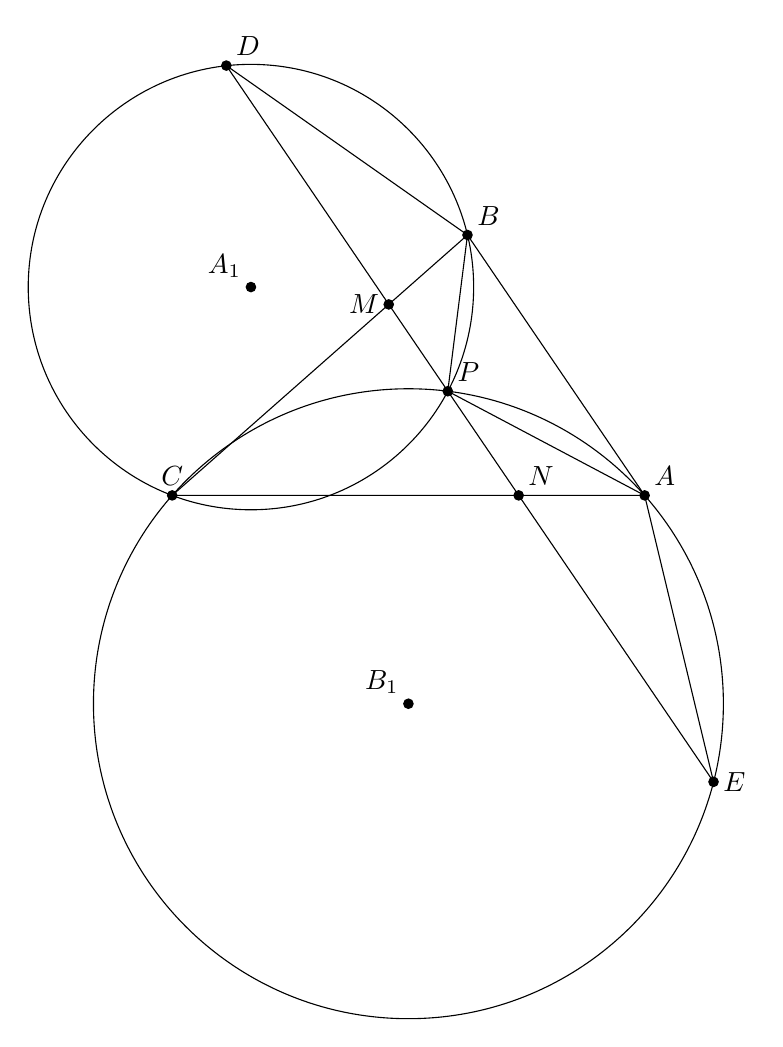
\begin{tikzpicture}
        \def\A{(6,0)}
        \def\B{(3.75,3.3071891)} 
        \def\C{(0,0)}
        \def\P{(3.5,1.3228756)} 
        \def\D{(0.6875,5.4586)} 
        \def\E{(6.875,-3.637908)} 
        \def\M{(2.75,2.42527203)}
        \def\N{(4.4,0)}
        \def\Aa{(1,2.64575)}
        \def\Bb{(3,-2.64575)}
        \filldraw \A circle (0.06) node[above right] {$A$};
        \filldraw \B circle (0.06) node[above right] {$B$}; 
        \filldraw \C circle (0.06) node[above] {$C$}; 
        \filldraw \P circle (0.06) node[above right] {$P$}; 
        \filldraw \D circle (0.06) node[above right] {$D$}; 
        \filldraw \E circle (0.06) node[right] {$E$}; 
        \filldraw \M circle (0.06) node[left] {$M$}; 
        \filldraw \N circle (0.06) node[above right] {$N$}; 
        \filldraw \Aa circle (0.06) node[above left] {$A_1$};
        \filldraw \Bb circle (0.06) node[above left] {$B_1$};
        \draw (3,-2.64575) circle (4);
        \draw (1,+2.645751) circle (2.82842);
        \draw \B -- \D -- \E -- \A -- \B -- \C -- \A -- \P -- \B;
        \end{tikzpicture}
    \end{figure}

    We claim $P$ is the incenter of $\triangle ABC$. By arc lengths, $\angle{PA'B} = 2 \angle BCP$ and since $A'P = A'B$ we have $\angle A'PB = 90 - \angle BCP \iff \angle APB = 90 + \angle BCP$.
    However, doing this to the circle centered at $B'$ gives $\angle APB = 90 + \angle ACP \iff \angle ACP = \angle BCP = \frac{\angle C}{2}$ and $\angle APB = 90 + \frac{\angle C}{2}$.
    The locus of all points such that $\angle APB = 90 + \frac{C}{2}$ is $(AIB)$, which the $C$-angle bisector intersects twice, once at $I$ and once outside of $\triangle ABC$; since $P$
    is specified to be inside $\triangle ABC$ we conclude $P \equiv I$. \medskip

    Since $\angle AEP = \angle ACP = \frac{\angle C}{2}$ and $\angle CAP = \angle APE = \frac{\angle A}{2}$ we have $\triangle{EAP} \cong \triangle CPA$ by AAS;
    similarly $\triangle CPB \cong \triangle DBP$ so $DE = EP + DP = AC + AB = 11$. Also, the tangents to the incircle from $A$ have length $s - a = \frac{5}{2}$
    and $[ABC] = rs \iff r = \frac{\sqrt7}{2}$ so $AP = 2 \sqrt 2$. \boxed{1210202}
\end{solution}\bigskip

